%- HandOut Flag -----------------------------------------------------------------------------------------
\makeatletter
\@ifundefined{ifHandout}{%
  \expandafter\newif\csname ifHandout\endcsname
}{}
\makeatother

%- D0cum3nt ----------------------------------------------------------------------------------------------
\documentclass[beamer,10pt]{standalone}   
%\documentclass[beamer,10pt,handout]{standalone}  \Handouttrue  

\ifHandout
	\setbeameroption{show notes} %print notes   
\fi

	
%- Packages -------------------------------------------------------------------------------------------
\usepackage{custom-style}
\usetikzlibrary{positioning}
\usepackage{multicol}
\usepackage{stmaryrd}

%--Beamer Style----------------------------------------------------------------------------------------
\usetheme{toninus}
\usepackage{animate}
\usetikzlibrary{positioning, arrows}
\usetikzlibrary{shapes}

%--Custom command----------------------------------------------------------------------------------------
\providecommand{\pairing}{\langle\cdot,\cdot\rangle}
\providecommand{\vHam}{\mathscr{v}}

\begin{document}
\outline


%-------------------------------------------------------------------------------------------------------------------------------------------------
\subsection{(Multi)-symplectic geometry: mechanical perspective}
%-------------------------------------------------------------------------------------------------------------------------------------------------
\begin{frame}{Symplectic geometry (mechanical perspective)}
\begin{columns}[T]
	\begin{column}{.50\linewidth}
		\centering
		\textit{ "geometric approach" to mechanics \dots}
		%
		\begin{columns}
			\begin{column}{.60\linewidth}
				\begin{center}
					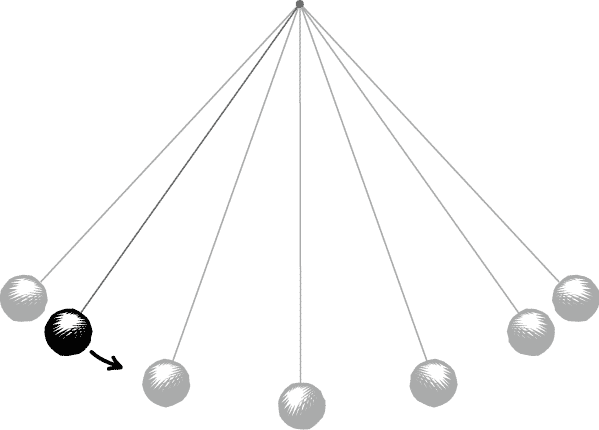
\includegraphics[width=0.6\linewidth]{Pictures/pendulum13}			
				\end{center}
			\end{column}	
			\begin{column}{.40\linewidth}
				\begin{center}
					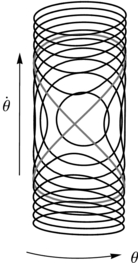
\includegraphics[width=0.45\linewidth]{Pictures/pendulum-phase-space}			
				\end{center}
			\end{column}	
		\end{columns}
		%
		\begin{defblock}[Symplectic Manifold]
			\vspace{-1em}
			\includestandalone[width=1\textwidth]{Pictures/Figure_sym}	
		\end{defblock}
		%
		\pause
		\begin{exblock}[$M = T^\ast Q$ is symplectic]
			with $\omega = d \theta $ given by
			$$ \left.\theta\right\vert_{(q,p)} (v) = p (\pi_\ast v) ~.$$
		\end{exblock}
		%
		\pause
		\vspace{1em}
		\centering
		\textit{ based on the notion of "states".}		
	\end{column}
	\onslide<1->{\vrule{}}
	\pause
	\begin{column}{.50\linewidth}
		\centering
		\textit{ "algebraic approach" to mechanics \dots}
		\vspace{.5em}	
		\begin{defblock}[Classical Observables]
			Unital, associative, commutative algebra $C^\infty(M)$.
		\end{defblock}
		%
		\vspace{.5em}
		\pause
		\begin{defblock}[Hamiltonian vector fields]
			$v_f \in \mathfrak{X}(M)$ such that:
			$$\iota_{v_f} \omega = -df \quad \text{(exact)}$$ %$\in B^1(M)$
			\small$v_f$ = \emph{Ham.v.f. pertaining to $f\in C^\infty(M)$}.
		\end{defblock}
		%
		\begin{defblock}[Poisson Algebra of Observables]
			$C^\infty(M)$ is a Poisson algebra with
			$$\{f,g\} = \iota_{v_g} \iota_{v_f} \omega = \omega(v_f,v_g) ~.$$
		\end{defblock}
		%
		\pause
		\vspace{.8em}
		\centering
		\textit{ based on the notion of "meaurable quantities".}						
	\end{column}
\end{columns}
\end{frame}
\note[itemize]{
	\footnotesize

	\item We work in the framework of multisymplectic geometry which is one of the possible generalizations of the well-established field of symplectic geometry.
	
	\item To recall what symplectic geometry is let me assume a particular point of view: mechanics.
	\\
	Idea:"
	Symplectic geometry is a branch of differential geometry studying symplectic manifolds; it originated as a formalization of the mathematical apparatus of classical mechanics and geometric optics."{\href{https://ncatlab.org/nlab/show/symplectic+geometry}{nlab}}
	
	Namely, a sym. mfd. is the geometric structure encoding the phase space of conservative, ordinary, classical, mechanical systems.
	
	\item $\theta$ = \emph{tautological 1-form}.
		$\theta$ evaluated at $p\in T^*Q$ in the fibre of $q\in Q$ and contracted with $v$ coincides with the form $p$ evaluated at $q$ and contracted with the push forward of $v$.
	
	\item We identify a special class of vector fields.
		Out of them one can define a Lie bracket.
	
	\item Poisson is a Lie algebra with the extra property of compatibility with the associative product (Leibniz rule)
	
	\item take away message: geometric (based on "states") vs algebraic (based on "measurable quantities").7
}
%-------------------------------------------------------------------------------------------------------------------------------------------------


%-------------------------------------------------------------------------------------------------------------------------------------------------
\begin{frame}[t]{From Symplectic to MultiSymplectic (mechanical perspective)}
	\begin{block}{Historical motivation}
		Mechanics: geometrical foundations of \textit{(first-order)} field theories.
		\begin{itemize}
		 \item[•] Kijowski, W. Tulczyjew \cite{Kijowski1979}; %(1979)
		 \item[•] Cariñena, Crampin, Ibort \cite{Carinena1991b};% (1991)
		 \item[•] Gotay, Isenberg, Marsden, Montgomery \cite{Gimmsy1};%(1998)
		 \\ $\cdots$
		\end{itemize}
	\end{block}
	\vfill
	\pause
	\tcbset{colback=white,
		colbacktitle=white,
		colframe=red!70!black,
		boxrule=1pt,
		colupper=red!70!black,
		arc=15pt}
	\begin{tcolorbox}[enhanced,frame hidden,borderline={0.5pt}{0pt}{red,dashed}]
		\color{red}
		\begin{columns}[T]
			\begin{column}{.20\linewidth}
				\begin{center}
					\huge
					\faWarning
				\end{center}
			\end{column}			
			\begin{column}{.60\linewidth}
				\vspace{-.4em}
				\begin{center}
					The lack of a satisfactory notion of observables hindered the spread of this formalism.
				\end{center}
			\end{column}			
			\begin{column}{.20\linewidth}
				\begin{center}
					\huge
					\faWarning
				\end{center}
			\end{column}			
		\end{columns}
	\end{tcolorbox}
	\vfill
	\pause
	\begin{tcolorbox}[enhanced,frame hidden,borderline={0.5pt}{0pt}{blue,dashed}]
		\color{blue}
		\begin{columns}[T]
			\begin{column}{.20\linewidth}
				\begin{center}
					\huge
					\faQuestionCircle
				\end{center}
			\end{column}			
			\begin{column}{.60\linewidth}
				\begin{center}
					\vspace{-.4em}
					{Why observables are so crucial?\qquad \qquad Quantization!}	
				\end{center}
			\end{column}			
			\begin{column}{.20\linewidth}
				\begin{center}
					\huge
					\faQuestionCircle
				\end{center}
			\end{column}			
		\end{columns}
	\end{tcolorbox}




\end{frame}
\note[itemize]{
	\item Historically, the interest in multisymplectic manifolds, has been motivated by the need for understanding the geometrical foundations of first-order classical field theories.
	The key point is that, just as one can associate a symplectic manifold to an ordinary classical mechanical system (e.g. a single
point-like particle constrained to some manifold), it is possible to associate a multisymplectic
manifold to any classical field system (e.g. a continuous medium like a filament or a fluid). See frame Extra-\ref{Frame:Ms-Field-Mechanics} 
	\item Forger and Romero say: \emph{"The multisymplectic formalism is manifestly consistent with the basic principles of field theory, preserving full covariance, and it is mathematically rigorous because it uses well established methods from calculus on finite-dimensional manifolds. On the other hand, it does not seem to permit any obvious definition of the Poisson bracket between observables. Even the question of what mathematical objects should represent physical observables is not totally clear and has in fact been the subject of much debate in the literature. Moreover, the introduction of n conjugate momenta for each coordinate obscures the usual duality between canonically con- jugate variables (such as momenta and positions), which plays a fundamental role in all known methods of quantization.A definite solution to these problems has yet to be found."}
	
}
%-------------------------------------------------------------------------------------------------------------------------------------------------

%-------------------------------------------------------------------------------------------------------------------------------------------------
\subsection{Observability}
%-------------------------------------------------------------------------------------------------------------------------------------------------
\begin{frame}{Observables in $n$-plectic geometry}
	%
	\begin{defblock}[Hamiltonian $(n-1)$-forms]
		\begin{displaymath}
			\Omega^{n-1}_{ham}(M,\omega) 	:=
			\biggr\{ \sigma \in  \Omega^{n-1}(M) \; \biggr\vert \; 
				\exists \vHam_\sigma \in \mathfrak{X}(M) ~:~ 
				\tikz[baseline,remember picture]{\node[rounded corners,
                        fill=orange!5,draw=orange!30,anchor=base]            
            			(target) {$d \sigma = -\iota_{\vHam_\sigma} \omega$ };
            	}				
				~\biggr\} 
			\end{displaymath}
	\end{defblock}

	\pause
		\tikz[overlay,remember picture]
		{
			\node[rounded corners,
                 fill=orange!5,draw=orange!30,anchor=base]
            	 (base) at ($(current page.north east)-(2,1)$) [rotate=-0,text width=3.5cm,align=center] {\footnotesize{\textcolor{red}{Hamilton-DeDonder-Weyl \\equation}}};
		}	
	\begin{tikzpicture}[overlay,remember picture]
    	\path[->] (base.south) edge[bend right,red](target.north);
    \end{tikzpicture}
	%
	\vspace{-2em}
	\begin{columns}[T]
		\pause
		\setlength{\belowdisplayskip}{5pt}
		\begin{column}{.50\linewidth}
			%
			\begin{thmblock}[Observables $L_\infty$-algebra]
				$\Omega^{n-1}_{ham}(M,\omega)$ endowed with
				\vspace{-.5em}
				\begin{displaymath}
					\lbrace \sigma_1, \sigma_2 \rbrace =			
					~ - \iota_{\vHam_1}\iota_{\vHam_2} \omega 
				\end{displaymath}			
				can be "completed" to a \\ $L_\infty-algebra$.
			\end{thmblock}
			%
			\pause
			\begin{itemize}
				\item[\cmark] Skew-symmetric;
				\item[\xmark] multiplication of observables;
				\item[\xmark] Jacobi equation;
				%\\ \hspace*{4.25em} full-fledged Jacobi equation;
				\item[\smark] Jacobi equation \emph{up to homotopies}.
			\end{itemize}				
		\end{column}	
		%
		\onslide<1->{\vrule{}}
		%
		\pause
		\begin{column}{.50\linewidth}
			\begin{thmblock}[Observables Leibniz algebra]
				$\Omega^{n-1}_{ham}(M,\omega)$ endowed with
				\vspace{-.5em}
			\begin{displaymath}
				\llbracket \sigma_1, \sigma_2 \rrbracket =
				~ \mathcal{L}_{\vHam_1} \sigma_2
				~.					
			\end{displaymath}		
				can be "completed" to a \\ DG-Leibniz algebra.
			\end{thmblock}	
			%
			\pause
			\begin{itemize}
				\item[\xmark] Skew-symmetric;
				\item[\xmark] multiplication of observables;
				\item[\cmark] Jacobi equation;
				\item[\smark] Skew-symmetric \emph{up to homotopies}.
			\end{itemize}	
		\end{column}	
	\end{columns}
\end{frame}
\note[itemize]{
 \item See \cite[\S 7.2]{Rogers2010} about the comparison of these two algebraic structures.
 \item Notice that the failure of skew-symmetricity is measured by
 \begin{align*}
 	A(\sigma_1,\sigma_2) 
 	=&~
 	 2~\llbracket \sigma_1, \sigma_2\rrbracket +  \llbracket \sigma_2, \sigma_1\rrbracket
 	 \\
 	 =&~ d \circ\langle\sigma_1,\sigma_2\rangle_+
 \end{align*}
 (Compare with the \href{https://en.wikipedia.org/wiki/Courant_bracket\#Dorfman_bracket}{Dorfmann bracket}.)
 
 \item Notice that the antisymmetrization of $\llbracket \cdot, \cdot \rrbracket$ equates $\lbrace \cdot,\cdot \rbrace$ modulo homotopy:
 \begin{align*}
  \llbracket \sigma_1,\sigma_2 \rrbracket  \circ 	\mathcal{A}
  =&~
  \frac{\mathcal{L}_{\vHam_1}\sigma_2 - \mathcal{L}_{\vHam_2}\sigma_1}{2} 
  \\
  =&~ 
  \frac{1}{2}( d (\iota_{\vHam_1}{\sigma_2} - \iota_{\vHam_2}{\sigma_1} )
  +\frac{1}{2}(-\iota_{\vHam_1}\iota_{\vHam_2}\omega + \iota_{\vHam_2}\iota_{\vHam_1}\omega) 
  \\
  =&~
  \lbrace \sigma_1, \sigma_2 \rbrace + d \circ \langle\sigma_1,\sigma_2\rangle_-
  \\
  =&~
  [\sigma_1,\sigma_2]_\omega
 \end{align*}
 where the last bracket is given by the Vinogradov algebroid Binary bracket.
}
%-------------------------------------------------------------------------------------------------------------------------------------------------

%------------------------------------------------------------------------------------------------------
\begin{frame}{Scope of the talk}
	%
	\centering
	\begin{tikzpicture}
		\node [draw,ellipse callout,red, minimum height=10em,minimum width=30em,callout relative pointer={(-2,-.5)}] (L1) {};
		\node [text width=25em,text centered] (L2) {
			\textcolor{red}{Broad \emph{general} question:}
			\\
			\medskip
			What is the corresponding	 "correct" notion of observables in multisymplectic geometry?	
		};
	\end{tikzpicture}
	\vfill
	\pause
	\begin{tikzpicture}
		\node [draw,blue,ellipse callout, minimum height=10em,minimum width=30em,callout relative pointer={(2,-.5)}] (L1) {};
		\node [text width=25em,text centered] (L2) {
			\textcolor{blue}{Specific \emph{technical} question}:
			\\
			\medskip
			How the compatibility diagram between \emph{gauge transformation}
			and \emph{comomentum maps} extends to the $n$-plectic case?
		};
	\end{tikzpicture}
\end{frame}
\note[itemize]{
	\item Non ho una risposta soddifacente alla domanda generale. Bisogna procedere per gradi.
	\item l'obbiettivo di questo lavoro con Marco è di stabilire quanto della seguente situazione si estende nel caso multisimplettico.
	\item It is possible to relate the observables algebras of two gauge-related multisymplectic structures (in he same cohomology class)
}
%-------------------------------------------------------------------------------------------------------------------------------------------------



\end{document}